\lab{Complex Numbers}{Complex Numbers}
\label{Lab:complex_intro}

\objective{Visualize complex functions to estimate their zeros and poles.}

\section*{Polar Representation of Complex Numbers}

Any complex number $z = x+iy$ can be written in \emph{polar coordinates} as $re^{i\theta}$ where
\begin{itemize}
\item $r=\sqrt{x^2+y^2}$ is the magnitude of $z$, and
\item $\theta = \arctan(y/x)$ is the angle between $z$ and 0, as in Figure \ref{fig:polar_coords}.
\end{itemize}
Conversely, Euler's formula implies $re^{i\theta} = r\cos(\theta) + ir\sin(\theta)$. Then if we set $re^{i\theta}=x+iy$ and equate real and imaginary parts, we find $x=r\cos(\theta)$ and $y=r\sin(\theta)$.

\begin{figure}
\begin{tikzpicture}[dot/.style={circle,fill=black,minimum size=3pt,inner sep=0pt,
            outer sep=-1pt}, >=stealth', thick, xscale=1.4]

\draw[-](-.5,0)--(3,0);
\draw[-](0,-.5)--(0,3);

\draw[-, dashed, gray, anchor=east](2.6,2.3)--(0,2.3);
\node[draw=none]()at(-.3,2.3){$iy$};
\draw[-, dashed, gray, anchor=north ](2.6,2.3)--(2.6,0);
\node[draw=none]()at(2.6,-.3){$x$};

\draw[gray](.75,0) arc (0:45:.7 and .7);

\draw[-](0,0)--(2.6,2.3);
\node[dot,draw](point)at(2.6,2.3){};
\node[draw=none]()at(.9,.35){$\theta$};

\draw [decorate,decoration={brace,amplitude=10pt},rotate=-45, gray] (0,0) --(.2,3.45);
\node[draw=none]()at(.95,1.55){$r$};


\end{tikzpicture}
\caption{The complex number represented by the black dot equals both $x+iy$ and $re^{i\theta}$, when $\theta$ is written in radians.}
\label{fig:polar_coords}
\end{figure}

It is easy to convert between coordinate systems in NumPy, which uses the symbol \li{1j} for the complex number $i=\sqrt{-1}$.
\begin{lstlisting}
>>> import numpy as np
>>> from matplotlib import pyplot as plt
>>> z = 2 - 2*1j
\end{lstlisting}
Use \li{np.angle()} and \li{np.absolute()} to compute $\theta$ and $r$, respectively.
These functions also operate elementwise on NumPy arrays.
\begin{lstlisting}
>>> theta = np.angle(z)
>>> r = np.absolute(z)

# The function np.absolute() returns a value between -pi and pi.
>>> print r, theta
(2.8284271247461903, -0.78539816339744828)

# Check that z=re^(i*theta)
>>> np.allclose(z, r*np.exp(1j*theta))
True
\end{lstlisting}

\section*{Visualizing complex functions}
Suppose we wish to graph a function $f(z): \mathbb{C} \rightarrow \mathbb{C}$. 
The difficulty is that $\mathbb{C}$ has 2 real dimensions, so the graph of $f$ should use 4 real dimensions.
 Since we already have ways to visualize 3 dimensions, we should choose one dimension to ignore. 
 We will ignore the magnitude $r = |f(z)|$ of the output.

To visualize $f$, we will asign a color to each point $z \in \mathbb{C}$. 
The color will correspond to the angle $\theta$ of the output $f(z)$. 
As an example, we have plotted the identity function $f(z)=z$ in Figure \ref{fig:identity}.
As $\theta$ goes from 0 to $2\pi$, the colors cycle smoothly counterclockwise from red to green to purple and back to red.

This kind of plot uses rectangular coordinates in the domain and polar coordinates (or rather, just the $\theta$-coordinate) in the codomain.
Note that this kind of plot tells you nothing about $|f(z)|$.

You can create the plot in Figure \ref{fig:identity} as follows.
Begin by creating a grid of complex numbers.
We create the real and imaginary parts separately, and then use \li{np.meshgrid()} to turn them into a single array of complex numbers.
\begin{lstlisting}
>>> x = np.linspace(-1, 1, 401)
>>> y = np.linspace(-1, 1, 401)
>>> X, Y = np.meshgrid(x, y)
>>> Z = X + 1j*Y
\end{lstlisting}

Now we compute the angles of the points in \li{Z} and plot these using \li{plt.pcolormesh()} with the colormap \li{'hsv'}. 
This colormap is red at both ends, so that $0$ and $2 \pi$ will map to the same color.

\begin{lstlisting}
>>> plt.pcolormesh(X, Y, np.angle(Z), cmap='hsv')
>>> plt.show()
\end{lstlisting}


\begin{figure}
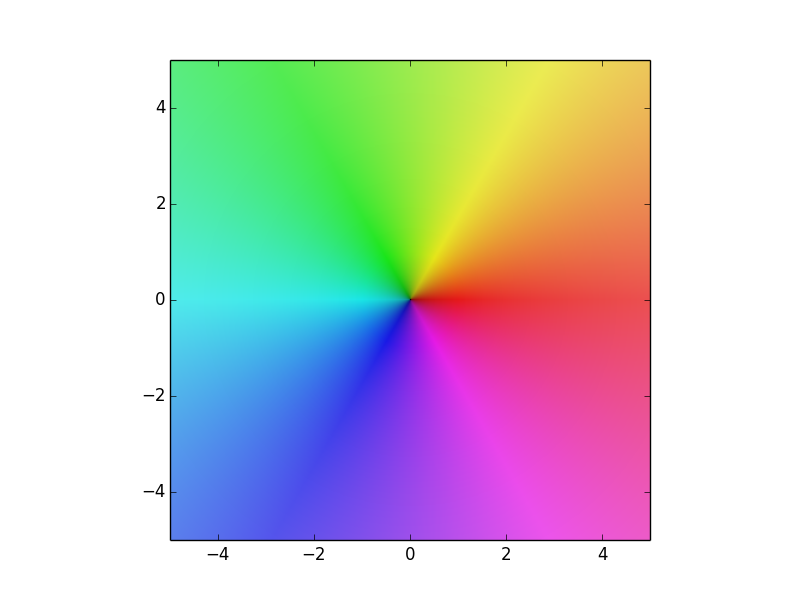
\includegraphics[width=.7\textwidth]{Identity.png}
\caption{Plot of $f: \mathbb{C} \rightarrow \mathbb{C}$ defined by $f(z)=z$. 
The color at each point $z$ represents the argument of $f(z)$.}
\label{fig:identity}
\end{figure}





\begin{problem}
Write the following function to plot any function from $\mathbb{C}$ to $\mathbb{C}$.
\begin{lstlisting}
def plot_complex(f, xbounds, ybounds, res=401):
    '''Plot the complex function f.
    
    INPUTS:
    f        - A function handle. Should represent a function 
    			from C to C.
    xbounds  - A tuple (xmin, xmax) describing the bounds on the real part 
    			of the domain.
    ybounds  - A tuple (ymin, ymax) describing the bounds on the imaginary 
    			part of the domain.
    res      - A scalar that determines the resolution of the plot. 
    			Defaults to 401.
    '''
\end{lstlisting}
When you call \li{plt.pcolormesh()} in this function, you should specify the keyword arguments \li{vmin} and \li{vmax}. 
These define which numbers should map to each end of the color scale. 
If you do not specify them, matplotlib will scale the colormap to fit your data exactly.

Check your function on the identity (graphed in Figure \ref{fig:identity}) and on the function $f(z) = \sqrt{z^2+1}$, which is graphed in Figure \ref{fig:check_plot}.
\begin{figure}[H]
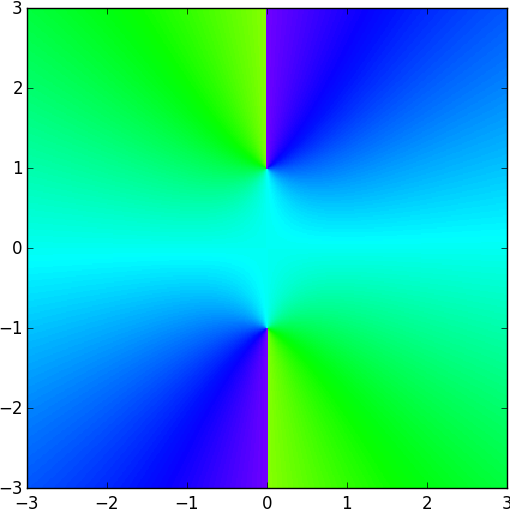
\includegraphics[width=.7\textwidth]{check_plot.png}
\caption{Plot of $\sqrt{z^2+1}$ on the domain $\{x+iy \mid x \in [-3,3] , \; y \in [-3,3]\}$ created by \li{plot_complex()}.}
\label{fig:check_plot}
\end{figure}

\end{problem}


\section*{Analyzing Complex Plots}

\subsection*{Zeros}

The plots created by your function \li{plot_complex()} are surprisingly informative.

\begin{problem}\label{prob:zeros}
\leavevmode
\begin{enumerate}
\item Use \li{plot_complex()} to plot the functions $z^2$, $z^3$, and $z^4$. What do you notice?
\item Plot $z^3 - iz^4 - 3z^6$ on the domain $\{x+iy \mid x \in [-1,1] , \; y \in [-1,1]\}$ (this plot is Figure \ref{fig:zeros}). 
Compare it to your plot of $z^3$, especially near the origin.
Based on these plots, what can you learn about the zeros of a function from its graph?
\end{enumerate}
\end{problem}

In Problem \ref{prob:zeros} you should have noticed when you plot $z^n$, the color circle around 0 repeats $n$ times. 
This is explained by looking at $z^n$ in polar coordinates:
\[
z^n = (re^{i \theta})^n = r^n e^{i(n\theta)}.
\]
Multiplying $\theta$ by a number greater than $1$ compresses the graph along the ``$\theta$-axis'' by a factor of $n$. 
Compare this to replacing $f(x)$ with $f(nx)$ when $f$ is a function from $\mathbb{R}$ to $\mathbb{R}$.

From Problem \ref{prob:zeros} you should also have noticed that the plot of $z^3 - iz^4 - 3z^6$ looks a lot like the plot of $z^3$ near the origin.
This is because when $z$ is very small, $z^4$ and $z^6$ are much smaller than $z^3$, and so the behavior of $z^3$ dominates the function.

In general, $f(z)$ has a \emph{zero of order $n$ at $z_0$} if the Taylor series of $f(z)$ centered at $z_0$ can be written as 
\[
f(z) = \sum_{k=n}^{\infty} a_k(z-z_0)^k \qquad \text{with} \; a_n \neq 0.
\]
In other words, $f(z) = a_n(z-z_0)^n + a_{n+1}(z-z_0)^{n+1} + \ldots$. 
In a small neighborhood of $z_0$, the quantity $|z-z_0|^{n+k}$ is much smaller than $|z-z_0|^n$, and so the function behaves like $a_n(z-z_0)^n$.
This explains why you can estimate the order of a zero by counting the number of times the colors circle a point (see Figure \ref{fig:zeros}).

\begin{figure}
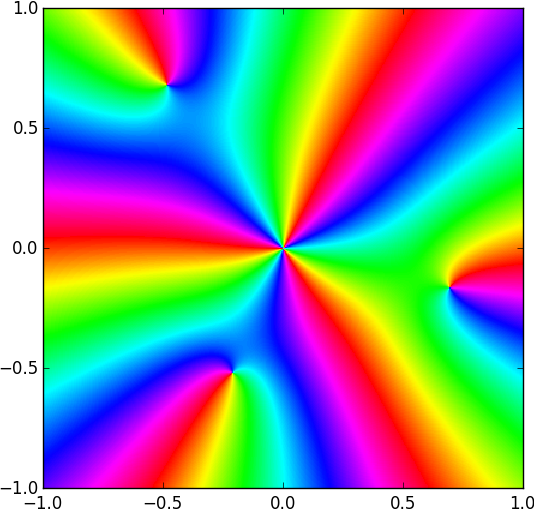
\includegraphics[width=.7\textwidth]{zeros.png}
\caption{Plot of $f(z)=z^3 - iz^4 - 3z^6$ on the domain $\{x+iy \mid x \in [-1,1] , \; y \in [-1,1]\}$.
From this plot we see that $f(z)$ has a zero of order 3 at the origin, and 3 zeros of order 1 scattered around it. 
This accounts for the 6 roots of $f(z)$ that are guaranteed to exist by the Fundamental Theorem of Algebra.}
\label{fig:zeros}
\end{figure}


\subsection*{Poles}

The plots created by \li{plot_complex()} can also tell us about the poles of a function.

\begin{problem}\label{prob:poles}
\leavevmode
\begin{enumerate}
\item Use \li{plot_complex()} to plot the function $f(z) = 1/z$. 
Compare this to the plot of $f(z)=z$ in Figure \ref{fig:identity}.
What is the difference?
\item Plot $z^{-2}$, $z^{-3}$, and $z^2+iz^{-1}+z^{-3}$ on the domain $\{x+iy \mid x \in [-1,1] , \; y \in [-1,1]\}$. 
Compare the plots of the last two functions near the origin.
Based on these plots, what can you learn about the poles of a function from its graph?
\end{enumerate}
\end{problem}

In Problem \ref{prob:poles} you should have noticed that in the graph of $1/z$, the colors cycle around 0 in the opposite direction from the graph of the identity map.
Again this can be explained by looking at the polar representation:
\[
z^{-n} = (re^{i \theta})^{-n} = r^{-n} e^{i(-n\theta)}.
\]
The minus-sign on the $\theta$ reverses the direction of the colors, and the $n$ makes them repeat $n$ times.

In general, a function has a \emph{pole of order n} at $z_0$ if its Laurent series on a punctured neighborhood of $z_0$ is
\[
f(z) = \sum_{k=-n}^\infty a_k(z-z_0)^k  \qquad \text{with} \; a_{-n} \neq 0.
\]
In other words, $f(z) = a_{-n}(z-z_0)^{-n}+a_{-n+1}(z-z_0)^{-n+1} + \ldots$.
Since $|z-z_0|^{-n+k}$ is much smaller than $|z-z_0|^{-n}$ when $|z-z_0|$ is small, near $z_0$ the function behaves like $a_{-n}(z-z_0)^{-n}$.
This explains why you can estimate the order of a pole by counting the number of times the colors circle a point in the ``backwards direction.''

Finally, a function has an \emph{essential pole} at $z_0$ if its Laurent series in a punctured neighborhood of $z_0$ requires infinitely many terms with negative exponents.
For example, 
\[
e^{1/z} = \sum_{k=0}^{\infty}\frac{1}{n! z^n} = 1+\frac{1}{z}+\frac{1}{2}\frac{1}{z^2}+\frac{1}{6}\frac{1}{z^3}+\ldots.
\]
The plot of $f(z) = e^{1/z}$ is in Figure \ref{fig:essential_singularity}. 
Here, you can see that the colors circle around an essential singularity infinitely many times.

\begin{figure}
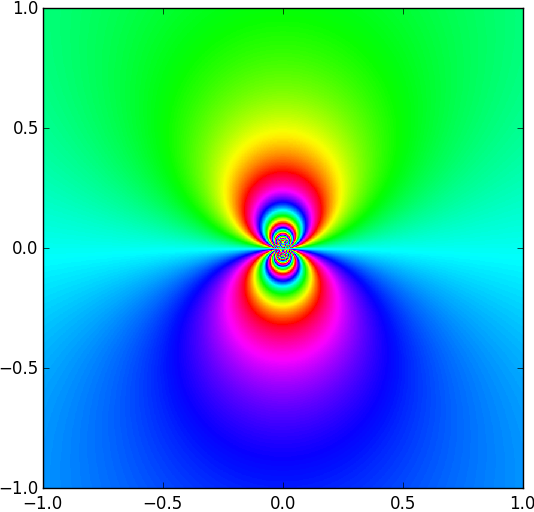
\includegraphics[width=.7\textwidth]{essential_pole.png}
\caption{Plot of $e^{1/z}$ on the domain $\{x+iy \mid x \in [-1,1] , \; y \in [-1,1]\}$.
The colors circle clockwise around the origin because it is a singularity, not a zero.
Because the singularity is essential, the colors repeat infinitely many times.}
\label{fig:essential_singularity}
\end{figure}

\subsection*{Using plots to estimate poles and zeros}
To summarize, you can use the plot of a complex function to estimate its poles and zeros with the following rules.
\begin{itemize}
\item Colors circle around zeros in the ``forwards direction''.
\item Colors circle around poles in the ``backwards direction''.
\item The number of times the colors repeat equals the order of the zero or pole.
\end{itemize}

\begin{problem}\label{prob:findpz}
Plot these functions on the domains given and estimate the number and order of their poles and zeros.
\begin{itemize}
\item $f(z) = e^z$ on $\{ x+iy \mid x \in [-8,8], \; y \in [-8,8]\}$
%\item $z^2-2z^7+2z^6-4z^5+2z^4-2z^3-5z^2+4z-4$ from $x \in [-2.5,2.5]$ and $y \in [-2.5,2.5]$ 
\item $f(z) = \tan(z)$ on $\{x+iy \mid x \in [-8,8], \; y \in [-8,8]\}$
\item $f(z) = \frac{16z^4+32z^3+32z^2+16z+4}{16z^4-16z^3+5z^2}$ on $\{x+iy \mid x \in [-1,1], \; y \in [-1,1]\}$
%\item $f(z) = \sin{\frac{1}{z}}$ on ${x+iy \mid x \in [-.8,.8], y \in [-.8,.8]\}$
\end{itemize}
\end{problem}

One useful application of complex plots is to estimate the zeros of polynomials and their multiplicity.

\begin{problem}\label{prob:find_roots}
Use complex plots to determine the multiplicity of the zeros of each of the following polynomials.
Use the Fundamental Theorem of Algebra to ensure that you have found them all.
\begin{enumerate}
\item $-2z^7+2z^6-4z^5+2z^4-2z^3-4z^2+4z-4$
\item $z^7 + 6z^6 - 131z^5 - 419z^4 + 4906z^3 - 131z^2 - 420z + 4900$
\end{enumerate}
\end{problem}

Plotting functions is not a substitute for rigorous mathematics. 
Often, plots can be deceptive.

\begin{problem}\label{prob:caution}
\leavevmode
\begin{enumerate}
\item This example shows that sometimes you have to ``zoom in'' to see all the information about a pole.
\begin{enumerate}
\item Plot the function $f(z) =\sin( \frac{1}{100z})$ on the domain $\{x+iy \mid x \in [-1,1],\; y \in [-1,1]\}$.
What might you conclude about this function?
\item Now plot $f(z)$ on $\{x+iy \mid x \in [-.01,.01], \; y \in [-.01,.01]\}$.
Now what do you conclude about the function?
\end{enumerate}
\item This example shows that from far away, two distinct zeros (or poles) can appear to be a single zero (or pole) of higher order.
\begin{enumerate}
\item Plot the function $f(z) = z+1000z^2$ on the domain $\{x+iy \mid x \in [-1,1], \; y \in [-1,1]\}$.
What does this plot imply about the zeros of this function?
\item Find the zeros of $f(z)$ using algebra.
\item Plot $f(z)$ on a domain that allows you to see the true nature of its zeros.
\end{enumerate}
\end{enumerate}
\end{problem}




















\begin{comment}

From these plots you can see the poles and zeros. The zeros are the black dots and the poles are the white dots on the plots. the order of the pole or zero can be read from the number of times the full set of colors show up around the pole or zero. As you can see from Figure \ref{fig:funcplot} $x^2-1$ has two zeros of order one at $1$ and $-1$. $x^4-\frac{1}{x^4}$ has eight zeros of order one and a pole of order four. 
For essential singularities the colors circle outward like in \ref{fig:e}, the plot of $e^\frac{1}{z}$.

\begin{figure}
\begin{subfigure}{.49\textwidth}
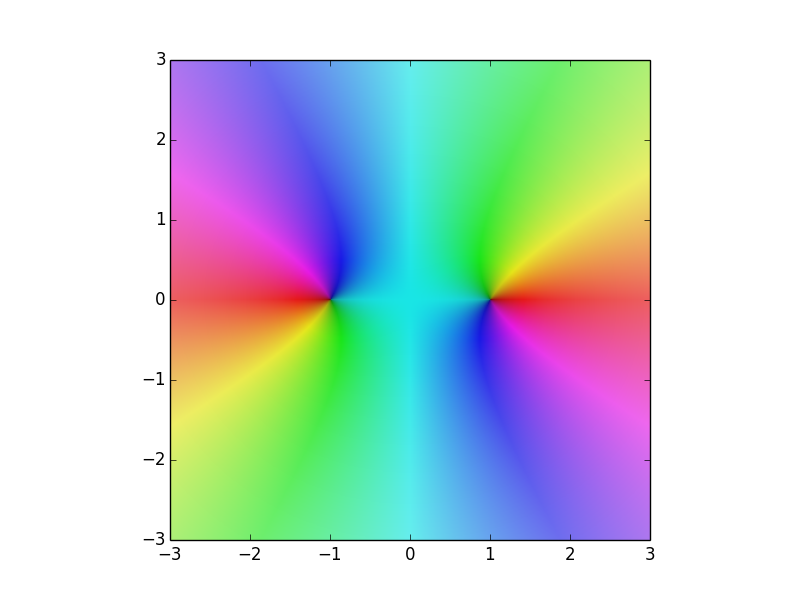
\includegraphics[width=\textwidth]{function.png}
\end{subfigure}
\begin{subfigure}{.49\textwidth}
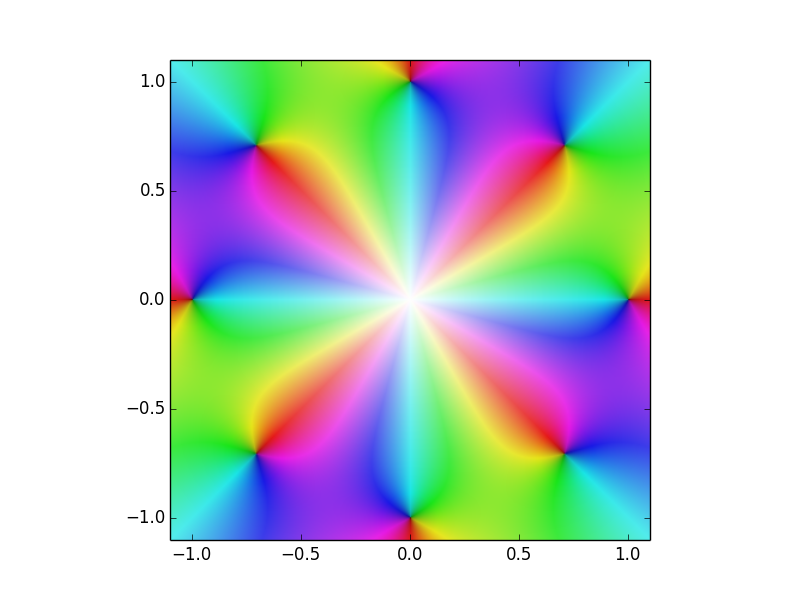
\includegraphics[width=\textwidth]{function2.png}
\end{subfigure}
\caption{Colorplot of the  function $x^2 - 1$ and $x^4-\frac{1}{x^4}$.}
\label{fig:funcplot}
\end{figure}

\begin{figure}
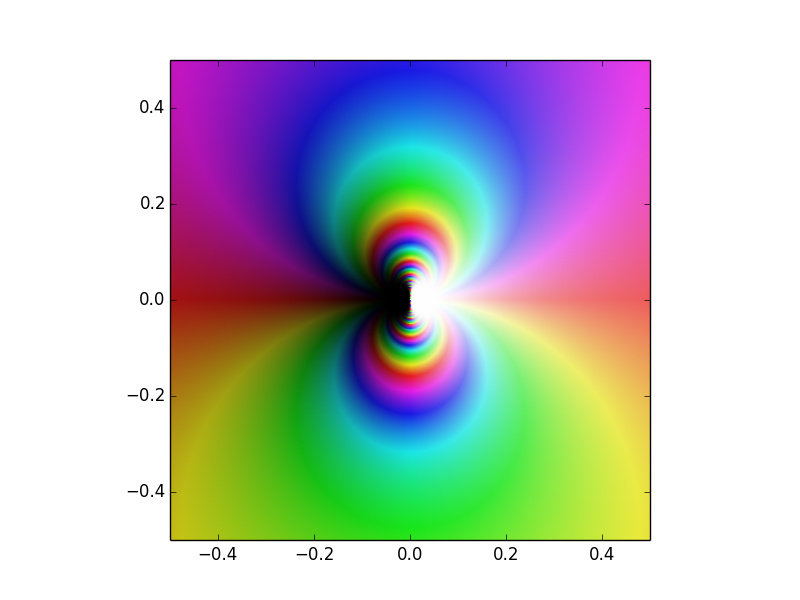
\includegraphics[width=\textwidth]{function1.png}
\caption{Color plot of the $e^\frac{1}{z}$.}
\label{fig:e}
\end{figure}

\begin{problem}

Plot the following functions and look at the plots. Write a function that prints out an estimate of the roots and/or poles and their order.
\begin{itemize}
\item Plot $e^z$ from $x \in [-8,8]$ and $y \in [-8,8]$, \item $z^2-2z^7+2z^6-4z^5+2z^4-2z^3-5z^2+4z-4$ from $x \in [-2.5,2.5]$ and $y \in [-2.5,2.5]$ 
\item Plot $\frac{16z^4+32z^3+32z^2+16z+4}{16z^4-16z^3+5z^2}$ from $x \in [-1,1]$ and $y \in [-1,1]$,
\item Plot $\sin{\frac{1}{z}}$ from $x \in [-.8,.8]$ and $y \in [-.8,.8]$,
\end{itemize}

\end{problem}




\section*{Multi-Valued Functions}

Another important topic in Complex Analysis is the study of multiple valued functions.
These functions arise as we consider the inverses of functions that are not strictly one to one on the complex plane.
A classic example is $\sqrt{x}$, which may take two values for every nonzero point of the complex plane.

In the Real numbers we worked with functions like this by simply restricting their output on a certain domain.
We can do a similar thing in the Complex plane.
Loosely speaking, such a restriction is called a branch.
Computationally we restrict the output to a single portion of the actual possible values of the multifunction.
We call inverse functions that have multiple values like this ``multi-valued functions" or ``multifuctions."
Numpy automatically restricts the output of multi-valued functions. So to get other cuts you have to modify the function to get the cut you want, like multiplying the output of the $\sqrt{x}$ by $-1$.
Figure \ref{fig:sqrt} shows the two cuts surfaces for $\sqrt{z}$ in the complex plane.

\begin{figure}
\begin{subfigure}{.49\textwidth}
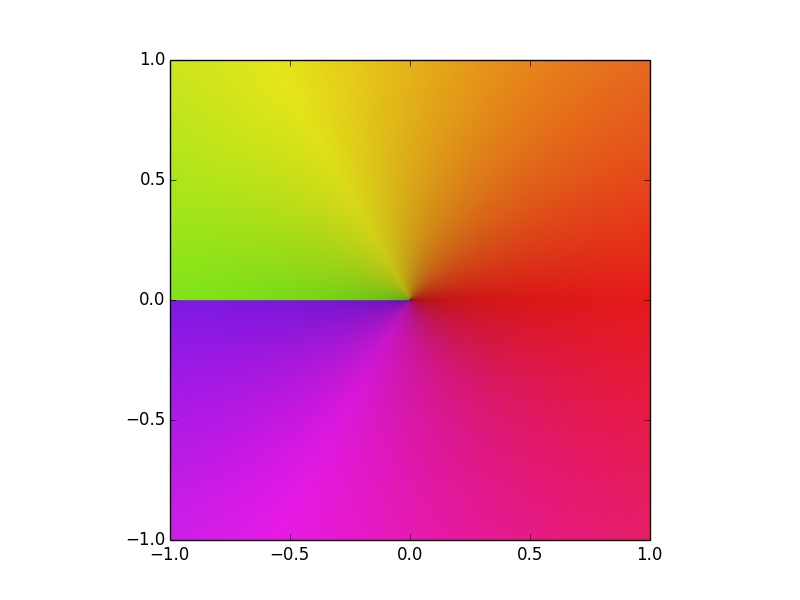
\includegraphics[width=\textwidth]{possqrt.png}
\end{subfigure}
\begin{subfigure}{.49\textwidth}
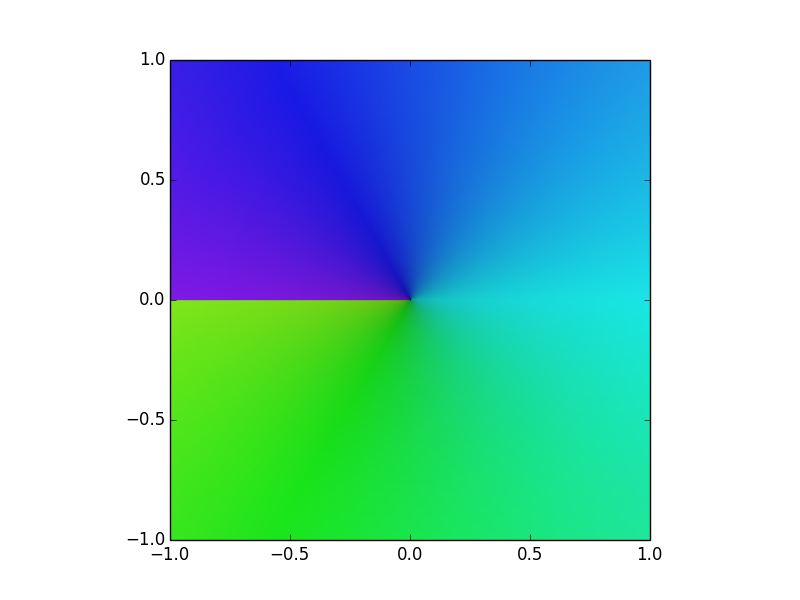
\includegraphics[width=\textwidth]{negsqrt.png}
\end{subfigure}
\caption{The positive and negative cut respectiviely of the function $\sqrt{z}$.}
\label{fig:sqrt}
\end{figure}

These are some very basic examples.
Another simple example is $\ln\left(z\right)$ which has a single value for the real part and infinitely many possible values for its imaginary part.
This is because for any complex $z\neq 0$, we have $e^z=e^{z+2n\pi}$ where $n$ is any integer.

\begin{problem}
Plot three cuts of $\ln\left(z\right)$ and$\arctan{x}$ on $x \in [-2,2]$ and $y \in [-2,2]$
\end{problem}

All three of these functions can be made analytic at almost any point, except at their singularities, but that depends on how we cut the domain to give it a single value.
When Integrating such functions, be careful about integrating across such cuts in the domain.


\begin{problem}
Write two functions, both accepting accept a natural number $n$.
Have one function plot the riemann surface for the real part $f(z)=\sqrt[n]{z}$ and the other plot the imaginary part.

Hint: Convert $z$ in $f(z)=\sqrt[n]{z}$ to polar form as $z=re^{\theta + 2k\pi}$
If you then plug this into $\sqrt[n]{z}$ the function takes the form
\[f(z)=\sqrt[n]{r} e^{i \frac{\theta + 2 \pi k}{n}}\]
Notice that here $f(z)$ has distinct values for $k = 0, 1, \dots, n-1$ a total of $n$ different values). Each value of $k$ corresponds to a different branch, which you can plot as $n$ separate surfaces.

If you use just one surface to plot each branch you will get erroneous vertical lines from jump discontinuities. Split each branch into two surfaces to get rid of these lines. You can investigate where the discontinuities occur by first plotting it as just one surface. The discontinuities happen at the same place for all $n$;
\end{problem}


\section*{Contour Integrals in the Complex Plane}

From multivariable calculus, you may recall that an integral may be taken along a path.
This is very similar to what we can be done in the complex plane.
Consider the function $f(z)$ on the complex plane.
Let $z=x+iy$.
Let $u$ and $v$ be the real and imaginary parts of $f$ respectively.
We integrate $f$ along some contour $C$ in the complex plane, beginning at $z=a$ and ending at $z=b$.
This integral may be written
\[\int_c f(z)dz\]
Parameterizing $z$, we have
\[\int_a^b f\left( c\left(t\right)\right) c'\left(t\right) dt\]
Expanding into real and imaginary parts (where $c\left(t\right) = x\left(t\right) + i y\left(t\right)$), we have
\[\int_a^b \left(u \left(c \left(t\right)\right) x'\left(t\right)-v\left(c \left(t\right)\right) y'\left(t\right)\right) dt + i \int_a^b\left(v \left(c \left(t\right)\right)x'\left(t\right)+u\left(c \left(t\right)\right) y'\left(t\right)\right) dt\]
We have now written this complex integral as the sum of two real valued integrals in $\mathbb{R}$.
Note that this implies that $\int_C f(z) dz$ may depend on the contour we choose and not just on the endpoints $a$ and $b$.

\begin{problem}
Write a function which takes a complex function $f(z)$, a contour parameterization $c(t)$ of a contour $c$, and the integration bounds on $t$ and returns the integral of $f$ along the contour $c$.
Use the numerical integration function \li{sympy.mpmath.quad} and the numerical derivative function \li{sympy.mpmath.diff} included in mpmath (which is, in turn, included as a submodule of sympy).
These functions already work for complex numbers.
To do something similar with the integration routines in SciPy, we would have to separate the function into real and imaginary parts, as is shown above.

Using the function you just defined, integrate the following functions along the following contours
\begin{itemize}
\item $\bar{z}$ counterclockwise along the unit ball starting and ending at $1$
\item $\bar{z}$ along a straight line from $0$ to $1+i$
\item $\bar{z}$ along the real axis from $0$ to $1$, then along the line from $1$ to $1+i$
\item $\bar{z}$ along the unit ball centered at $i$ from $0$ to $1+i$
\item $e^z$ counterclockwise along the unit ball starting and ending at $1$
\item $e^z$ along a straight line from $0$ to $1+i$
\item $e^z$ along the real axis from $0$ to $1$, then along the line from $1$ to $1+i$
\item $e^z$ along the unit ball centered at $i$ from $0$ to $1+i$
\end{itemize}
\end{problem}

Notice that, for a holomorphic function on a simply connected domain, the integrals from one point to another are not path dependent for any contours that lie within the domain.
An immediate consequence of the theorem is that for a complex function $f$, holomorphic on a simply connected domain $D$, and a contour $C$ lying entirely within $D$ which begins and ends at some point $a\in D$,
\[\int_C f(z)dz=0\]

The quadrature algorithms used in many of the integration algorithms work along a straight line between the integration bounds in the complex plane, so for holomorphic functions we should be able to use the integration function we wrote earlier.
For example, integrating $e^z$ from $-1-i$ to $1+i$ can be done numerically like this:
\begin{lstlisting}
from sympy import mpmath as mp
mp.quad(lambda z: mp.exp(z), (complex(-1, -1), complex(1, 1)))
\end{lstlisting}

\section*{The Cauchy Integral Formula}

Another major theorem in complex analysis is called Cauchy's Integral Formula (not to be confused with Cauchy's Integral Theorem).
It states that for a domain $D$ in the complex plane, containing some contour $C$ and the interior of $C$, for any $z_0$ in the interior of $C$,
\[f(z_0)=\frac{1}{2\pi i} \int_C \frac{f(z)}{z-z_0} dz\]

With more work, this theorem can be used to show that any function $f$ holomorphic on some domain $D$ is also infinitely differentiable on that domain.
In fact, the $n$th derivative of $f$ is given by the formula
\[f^{(n)}(z_0) = \frac{n!}{2\pi i} \int_C \frac{f(z)}{(z-z_0)^{n+1}} dz\]
This result is also important because it allows us to relate the value of $f$ on the inside of a contour to the value of $f$ on the contour itself.
In other words, the values of $f$ inside the contour depend only on the values of $f$ along the contour itself.
A related theorem (the Morera theorem) states that if some function $f$ is continuous on a domain $D$ and for every contour beginning and ending at the same point, the formula $\int_C f(z) dz = 0$ holds, then $f$ is holomorphic on $D$.

\begin{problem}
Using Cauchy's Integral Formula, write a python function which returns a callable function which evaluates a complex function $f$ along the interior of a contour $C$.
It should accept a callable function for the paramaterization of $C$, a callable function for the values of $f$ along $C$, and the bounds on the parameter used.
Assume in your function that $C$ begins and ends at the same point and that $f$ also begins and ends at the same value (so that $f$ is continous along $C$)
Try it out on simple functions like $e^x$ with complex values and compare what you get with what calling the functions normally gives you.
\end{problem}

Notice that in Cauchy's Integral Formula, we are integrating along a contour that begins and ends at the same point.
The function is also holomorphic at every point except $z_0$. At $z_0$ the integrand is undefined and has a singularity.
This integral around a singularity has some useful properties.
We will discuss these properties later on.

\end{comment}

\subsection*{Multi-valued functions}
Every complex number has two complex square roots, since if $w^2=z$, then also $(-w)^2=z$.
If $z$ is not zero, these roots are distinct.

Over the nonnegative real numbers, it is possible to define a continuous square root function.
However, it is not possible to define a continuous square root function over any open set of the complex numbers that contains 0.
This is intuitive after graphing $\sqrt{z}$ on the complex plane.

\begin{problem}
\begin{enumerate}
\item Use \li{plot_complex} to graph $f(z) = \sqrt{z}$.
Use \li{np.sqrt()} to take the square root.
What do you see?
\item Now plot $f(z) = -\sqrt{z}$ to see the ``other square root'' of $z$. What do you see?
\end{enumerate}
\end{problem}

Just as raising $z$ to a positive integer ``compresses the $\theta$-axis'', making the color wheel repeat itself $n$ times around 0, raising $z$ to a negative power \emph{stretches} the $\theta$-axis, so that only one $n^{th}$ of the color wheel appears around 0.
The colors at the ends of this $n^{th}$-slice are not the same, but they appear next to each other in the plot of $z^{-n}$.
This discontinuity will appear in every neighborhood of the origin. 


If your domain does not contain the origin, it is possible to define a continuous root function by picking one of the roots.


\section*{Appendix}
It is possible to visualize the argument and the modulus of the output of a complex function $f(z)$. 
One way to do so is to assign the modulus to a \emph{lightness} of color.
For example, suppose we have a complex number with argument 0, so it will map to red in the color plots described above.
If its modulus is very small, then we can map it to a blackish red, and if its modulus is large, we can map it to a whitish red.
With this extra rule, our complex plots will still be very much the same, except that zeros will look like black dots and poles will look like white dots (see Figure \ref{fig:example} for an example).

The code below implements the map we just described.
Be warned that this implementation does not scale well.
For example, if you try to plot a complex function whose outputs are all very small in modulus, the entire plot will appear black.


\begin{lstlisting}
import numpy as np
import matplotlib.pyplot as plt
from colorsys import hls_to_rgb

def colorize(z):
    ''' 
    Map a complex number to a color (or hue) and lightness.
    
    INPUT:
    z - an array of complex numbers in rectangular coordinates
    
    OUTPUT:
    If z is an n x m array, return an n x m x 3 array whose third axis encodes 
    (hue, lightness, saturation) tuples for each entry in z. This new array can 
    be plotted by plt.imshow().
    '''
    
    zy=np.flipud(z)
    r = np.abs(zy)
    arg = np.angle(zy)

    # Define hue (h), lightness (l), and saturation (s)
    # Saturation is constant in our visualizations
    h = (arg + np.pi)  / (2 * np.pi) + 0.5
    l = 1.0 - 1.0/(1.0 + r**0.3)
    s = 0.8

    # Convert the HLS values to RGB values.
    # This operation returns a tuple of shape (3,n,m).
    c = np.vectorize(hls_to_rgb) (h,l,s) 
    
    # Convert c to an array and change the shape to (n,m,3)
    c = np.array(c)  
    c = c.swapaxes(0,2)
    c = c.swapaxes(0,1)
    return c
\end{lstlisting}

The following code uses the \li{colorize()} function to plot  $\frac{z^2 - 1}{z}$. The output is Figure \ref{fig:example}.

\begin{lstlisting}
>>> f = lambda z :  (z**2-1)/z
>>> x = np.linspace(-.5, 1.5, 401)
>>> y = np.linspace(-1, 1, 401)
>>> X,Y = np.meshgrid(x,y)
>>> Z=f(X+Y*1j)
>>> Zc=colorize(Z)
>>> plt.imshow(Zc, extent=(-.5, 1.5, -1, 1))
>>> plt.show()
\end{lstlisting}

\begin{figure}
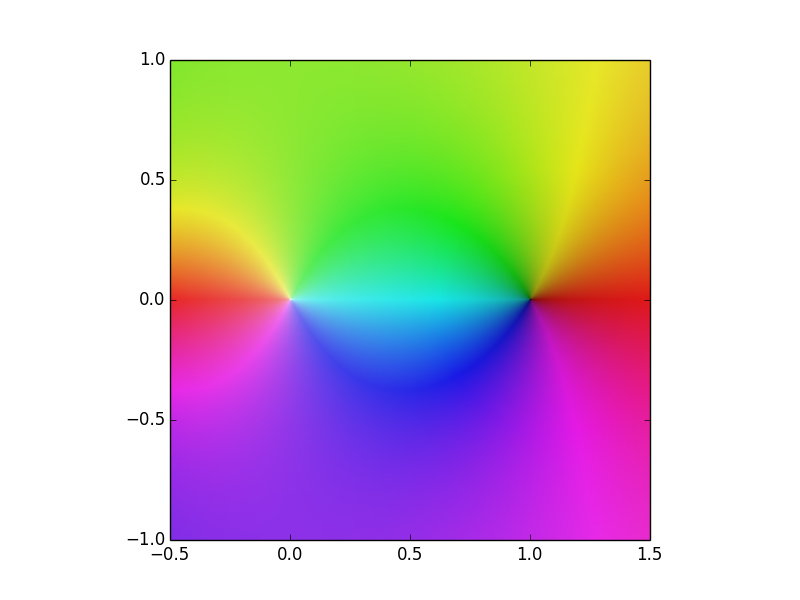
\includegraphics[width=\textwidth]{example.png}
\caption{Plot of the function $\frac{z^2 - 1}{z}$ created with \li{colorize()}.
Notice that the zero at 1 is a black dot and the pole at 0 is a white dot.}
\label{fig:example}
\end{figure}

